%!TEX root = ../report.tex
\documentclass[../report.tex]{subfiles}
\begin{document}
    \chapter{Evaluation and Results}
	This chapter presents the results of experiments whose implementation details were provided in the last chapter. Besides, the outcomes are systematically analyzed and evaluated.
	
	
	\section{Background}
	We conducted the first three experiments (A. patient-wise attribution map generation, B. composite face generation and C. syndrome-wise attribution map generation) on each of the 139 frequent syndrome classes in the GestaltMatcherDataBase (GMDB) dataset. Experimental artifacts from three of the syndromes were evaluated by an experienced clinical geneticist: Cornelia de Lange syndrome (CDLS), Williams syndrome (Williams Beuren syndrome) (WBS) and Hyperphosphatasia-intellectual disability syndrome or Hyperphosphatasia with Mental Retardation Syndrome (HPMRS). Therefore, analyses and discussions on experimental results mostly revolve around the three syndrome categories. Besides, some important findings from other syndromes are also provided. In this section, some background information regarding facial phenotypic features of the syndromes discussed in this chapter is given. 
	
	\subsubsection{Cornelia De Lange Syndrome}
		\begin{figure}[H]\label{fig_cdls_char}
		\centering
		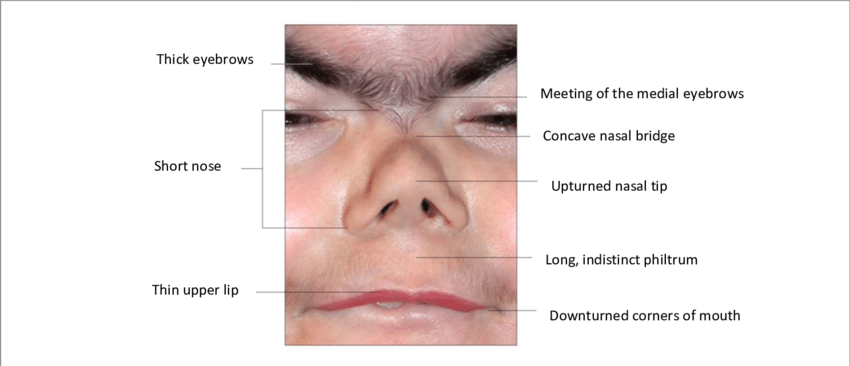
\includegraphics[scale=0.5, trim = 1cm 1cm 1cm 1cm, clip]{chapter6/cdls/cdls_ref.png}	
		\caption[Cardinal features of CDLS]{Cardinal facial features of CDLS. Source: \cite{kline2018diagnosis}}
	\end{figure}
	
	\begin{figure}[H]\label{fig_cdls}
		\centering
		\begin{subfigure}[b]{0.24\textwidth}
			\centering
			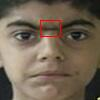
\includegraphics[width=\textwidth]{chapter6/cdls/0_3529.jpg}
		\end{subfigure}
		\begin{subfigure}[b]{0.24\textwidth}
			\centering
			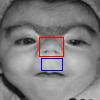
\includegraphics[width=\textwidth]{chapter6/cdls/9_2000.jpg}
		\end{subfigure}	
		\begin{subfigure}[b]{0.24\textwidth}
			\centering
			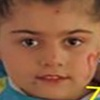
\includegraphics[width=\textwidth]{chapter6/cdls/33_3580.jpg}
		\end{subfigure}	
		\begin{subfigure}[b]{0.24\textwidth}
			\centering
			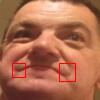
\includegraphics[width=\textwidth]{chapter6/cdls/117_3699.jpg}
		\end{subfigure}
		\caption[Instances of CDLS from GMDB dataset]{Instances of CDLS from GMDB dataset}
	\end{figure}
	
	\subsubsection{Williams Beuren Syndrome}
	\begin{figure}[H]\label{fig_williams_char}
	\centering
	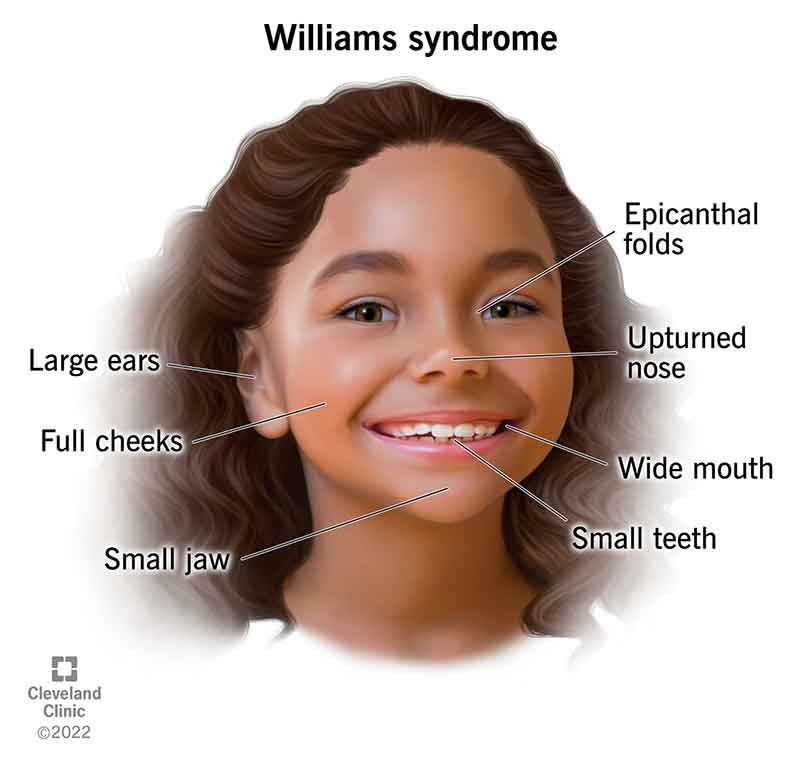
\includegraphics[scale=0.2]{chapter6/william/williams_syndrome_ref.jpg}	
	\caption[An animated characteristic face of WBS]{An animated characteristic face of WBS. Source: \url{https://my.clevelandclinic.org/health/diseases/15174-williams-syndrome}}
	\end{figure}
	
	\begin{figure}[H]\label{fig_williams}
		\centering
		\begin{subfigure}[b]{0.17\textwidth}
			\centering
			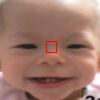
\includegraphics[width=\textwidth]{chapter6/william/4_37.jpg}
		\end{subfigure}
		\begin{subfigure}[b]{0.17\textwidth}
			\centering
			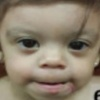
\includegraphics[width=\textwidth]{chapter6/william/4_73.jpg}
		\end{subfigure}	
			\begin{subfigure}[b]{0.17\textwidth}
			\centering
			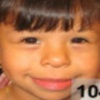
\includegraphics[width=\textwidth]{chapter6/william/33_111.jpg}
		\end{subfigure}	
			\begin{subfigure}[b]{0.17\textwidth}
			\centering
			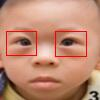
\includegraphics[width=\textwidth]{chapter6/william/130_36.jpg}
		\end{subfigure}	
			\begin{subfigure}[b]{0.17\textwidth}
			\centering
			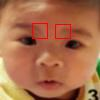
\includegraphics[width=\textwidth]{chapter6/william/164_35.jpg}
		\end{subfigure}	
	\caption[Instances of WBS from GMDB dataset]{Instances of WBS from GMDB dataset }
	\end{figure}





	\subsubsection{Hyperphosphatasia with Mental Retardation Syndrome}
	 
	 \begin{figure}[H]\label{fig_hpmrs}
	 	\centering
	 	\begin{subfigure}[t]{0.17\textwidth}
	 		\centering
	 		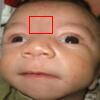
\includegraphics[width=\textwidth]{chapter6/hpmrs/2_499.jpg}
	 		\caption{Hypertelorism}
	 	\end{subfigure}
	 	\begin{subfigure}[t]{0.17\textwidth}
	 		\centering
	 		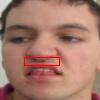
\includegraphics[width=\textwidth]{chapter6/hpmrs/15_1758.jpg}
	 		\caption{Short philtrum}
	 	\end{subfigure}	
	 	\begin{subfigure}[t]{0.17\textwidth}
	 		\centering
	 		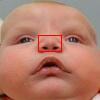
\includegraphics[width=\textwidth]{chapter6/hpmrs/17_1774.jpg}
			\caption{Short nose}
	 	\end{subfigure}	
	 	\begin{subfigure}[t]{0.17\textwidth}
	 		\centering
	 		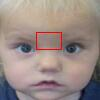
\includegraphics[width=\textwidth]{chapter6/hpmrs/20_888.jpg}
	 		\caption{Broad nasal bridge}
	 	\end{subfigure}	
	 	\begin{subfigure}[t]{0.17\textwidth}
	 		\centering
	 		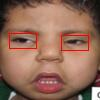
\includegraphics[width=\textwidth]{chapter6/hpmrs/33_1773.jpg}
	 		\caption{Upslanting palpebral fissures}
	 	\end{subfigure}	
	 	\caption[Instances of HPMRS from GMDB dataset]{Instances of HPMRS from GMDB dataset annotated with phenotypic facial features}
	 \end{figure}
	 
	 	\subsubsection{Coffin Siris syndrome}
	 
	 \begin{figure}[H]\label{fig_cfs}
	 	\centering
	 	\begin{subfigure}[t]{0.17\textwidth}
	 		\centering
	 		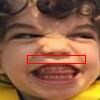
\includegraphics[width=\textwidth]{chapter6/cfs/5_1981.jpg}
	 		\caption{Short philtrum}
	 	\end{subfigure}
	 	\begin{subfigure}[t]{0.17\textwidth}
	 		\centering
	 		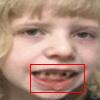
\includegraphics[width=\textwidth]{chapter6/cfs/6_810.jpg}
	 		\caption{Thin upper-lip vermilion and thich lower-lip vermilion }
	 	\end{subfigure}	
	 	\begin{subfigure}[t]{0.17\textwidth}
	 		\centering
	 		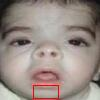
\includegraphics[width=\textwidth]{chapter6/cfs/17_2539.jpg}
	 		\caption{Small chin}
	 	\end{subfigure}	
	 	\begin{subfigure}[t]{0.17\textwidth}
	 		\centering
	 		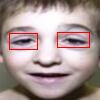
\includegraphics[width=\textwidth]{chapter6/cfs/20_2465.jpg}
	 		\caption{Downslanting palpebral fissures}
	 	\end{subfigure}	
	 	\begin{subfigure}[t]{0.17\textwidth}
	 		\centering
	 		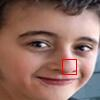
\includegraphics[width=\textwidth]{chapter6/cfs/46_1986.jpg}
	 		\caption{Broad nasal tip}
	 	\end{subfigure}	
	 	\caption[Instances of HPMRS from GMDB dataset]{Instances of CFS from GMDB dataset annotated with phenotypic facial features}
	 \end{figure}
	 
	 
    \section{Experiment A. Patient-wise Attribution Map Generation}
    
    \section{Experiment B. Composite Face Generation}
    Figure \ref{} contains composite faces of the top-ten syndrome classes by sample strength in 
    
    
    
    
    
    
    
    
    \section{Experiment C. Syndrome-wise Attribution Map Generation}


	\section{Experiment D. Dataset Imbalance - Explanation Quality Analysis}

    \section{Evaluation Summary}


\end{document}
